\section{Moshpit SGD}\label{sect:method}


Large-scale training with unreliable participants requires a protocol that is both communication-efficient and fault-tolerant. Unfortunately, existing methods have only  provide one of these properties. To better address our conditions, we propose Moshpit All-Reduce --- a fully decentralized averaging protocol that combines the efficiency of all-reduce and the fault tolerance of gossip-based averaging. 

The rest of this section is organized as follows:
\begin{itemize}
    \item Section~\ref{sect:method_algorithm} describes the protocol and proves its correctness and communication efficiency;
    \item Section~\ref{sect:method_convergence} provides the analysis of the protocol and proves exponential convergence rate for averaging and the rate matching the one of centralized Local-SGD for optimization;
    \item Section~\ref{sect:method_implementation_details} contains implementation details for training with heterogeneous compute nodes.
\end{itemize}

\subsection{Moshpit All-Reduce}
\label{sect:method_algorithm}

The core idea of Moshpit All-Reduce is that workers perform averaging in small independent groups. That way, a single failed participant would only affect his current group. In turn, the composition of each group should be chosen dynamically to converge in the least number of steps.
Ideally, if there are 9 peers with local parameters $\theta$, we can average them in 2 rounds, as demonstrated in Figure~\ref{fig:square_allreduce}:

\vspace{-4pt}
\noindent
\begin{minipage}{0.45\textwidth}
\centering
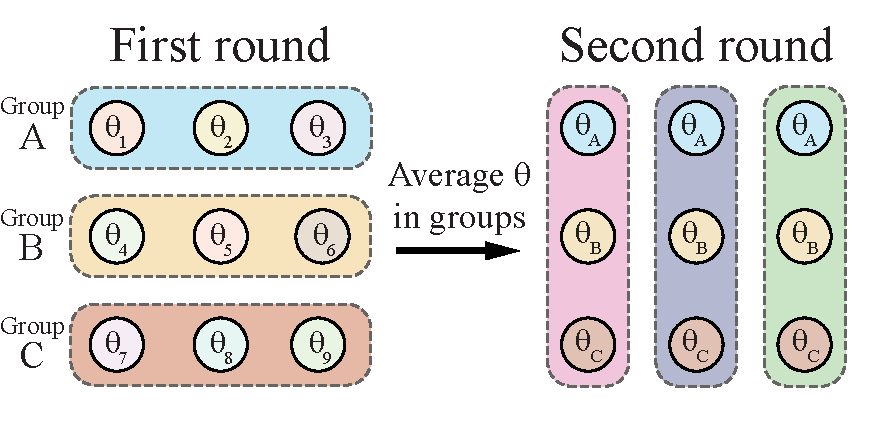
\includegraphics[width=\textwidth]{resources/moshpit.pdf}
\captionof{figure}{Example averaging order for 9 peers in 2 rounds. On each round, peers are split into 3 groups that run All-Reduce in parallel.}
\label{fig:square_allreduce}
\end{minipage}
\begin{minipage}{0.55\textwidth}
\begin{algorithm}[H]
\caption{Moshpit All-Reduce (for $i$-th peer)}
   \label{alg:moshpit}
\begin{algorithmic}[H]
   \STATE {\bfseries Input:} parameters $\{\theta_j\}_{j=1}^N$, number of peers $N$, $d$, $M$, number of iterations $T$, peer index $i$

   $\theta_{i}^0 := \theta_i$
   
   $C^0_i :=\texttt{get\_initial\_index(i)}$
   
   \FOR{$t \in 1 \dots T$}
     \STATE $\texttt{DHT}[C^{t-1}_i, t].\texttt{add}(\texttt{address}_i)$
     
     \STATE \texttt{Matchmaking()} // wait for peers to assemble
     
     \STATE $\texttt{peers}_t := \texttt{DHT}.\texttt{get}([C^{t-1}_i, t])$ 
     
     \STATE $\theta_{i}^t, c^t_i := \texttt{AllReduce}(\theta_{i}^{t - 1}, \texttt{peers}_t)$
     
     \STATE $C^t_i := (C^{t-1}_i\texttt{[1:]}, c^t_i)$  // same as eq. (1)
   \ENDFOR
   \STATE {\bfseries Return} $\theta^T_i$
\end{algorithmic}
\end{algorithm}
\end{minipage}

To achieve this in a decentralized system, we use Distributed Hash Tables (DHT) --- a decentralized key-value storage; \autoref{sect:post_related} contains its more detailed description. On each averaging round:
\begin{itemize}
    \item Each worker computes its group key $C_i$;
    \item Workers add their network addresses to the DHT key corresponding to $C_i$;
    \item Each worker can now fetch a full list of peers that have the same $C_i$ and run All-Reduce with those peers.
\end{itemize}

Unfortunately, the averaging structure from Figure~\ref{fig:square_allreduce} is impossible to maintain when participants are constantly joining, leaving, and failing. However, we can achieve equivalent results without global structure using a simple rule: \textit{if two peers were in the same group in round $t$, they must choose different groups in round $t {+} 1$.}

A natural way to enforce this rule is to take advantage of the chunk indices from Butterfly All-Reduce (see Figure~\ref{fig:butterfly_allreduce}). Recall that each worker accumulates a \textit{unique} chunk of parameters defined by an index $c_i$. By setting $C_i := c_i$, we can guarantee that any workers that were in the same group at a round $t$ will have different group indices in round $t {+} 1$.

This averaging scheme can be generalized to more than two dimensions in order to fit a larger number of peers or reduce the group size. For a $d$-dimensional hypercube, nodes should find groups of peers that they have not communicated with during $d {-} 1$ previous rounds. To that end, we define $C_i$ as tuples containing chunk indices from $d{-}1$ previous rounds ($t$ denotes the communication round):
\vspace{-2pt}
\begin{equation}
    C^t_i := (c^{t-d+1}_i, c^{t-d+2}_i, \ldots, c^{t }_i).
    \label{eq:group}
\end{equation}

The above intuition can be formalized with Algorithm \ref{alg:moshpit}.
Here, $N$ peers form a virtual $d$-dimensional grid with $M$ peers per row and average their parameters $\theta_i$ over $T$ rounds. $\texttt{DHT}[\cdot]$ is a shortcut for using the DHT to add or retrieve values for a given key. The  \texttt{Matchmaking} step corresponds to the decentralized matchmaking procedure that organizes active workers with the same index into groups, described in detail in ~\autoref{sect:matchmaking}. In turn, \texttt{AllReduce} denotes running all-reduce to compute the average $\theta$ in a given group. The \texttt{get\_initial\_index} function takes the peer index $i$ and returns $d{-}1$ integers
in range $[0, M)$ such that the size of initial groups does not exceed $M$.
This way, the groups formed on subsequent rounds will also have at most $M$ participants. One possible strategy is:

\vspace{-8pt}
\begin{equation}
    \texttt{get\_initial\_index}(i) = 
    \begin{pmatrix}
           \lfloor i / M^{d{-}1} \rfloor \Mod M \\
         \end{pmatrix}_{j\in \{1,\ \ldots,\ d\}}
    \label{eq:get_initial_index}
\end{equation}

If $N {=} M^d$ and there are no node/network failures, Algorithm~\ref{alg:moshpit} is equivalent to Torus All-Reduce~\cite{torus_allreduce}, achieving the exact average after $d$ rounds of communication (see Appendix~\ref{sect:equiv_to_torus}).
However, our typical use case is far from this perfect scenario; for example, some groups can have less than $M$ members. Furthermore, a peer might fail during all-reduce, causing its groupmates to skip a round of averaging. 
Still, Moshpit All-Reduce is applicable even in these conditions:
\begin{theorem}[Correctness]\label{thm:quality_of_avg_deterministic_vectors_0}
If all workers have a non-zero probability of successfully running a communication round and the order of $\texttt{peers}_t$ is random, then all local vectors $\theta^t_i$ converge to the global average with probability 1:
\vspace{-4px}
\begin{equation}
    \forall i, \Big|\Big|\theta^t_i - \frac1N \sum_i \theta^0_i\Big|\Big|^2_2 \xrightarrow[t\to\infty]{} 0.
\end{equation}
\end{theorem}\vspace{-16pt}
\begin{proof}[Proof (sketch, complete in Appendix~\ref{sect:correctness_proof})]
Running all-reduce with a subset of peers preserves the invariant $\frac1N \sum_i \theta^t_i=\frac1N \sum_i \theta^{t-1}_i$ and reduces the deviation of $\theta^t_i$ from the overall average.
\end{proof}\vspace{-6pt}

\textbf{Complexity.} The matchmaking protocol is implemented over Kademlia DHT~\cite{kademlia}, meaning that each read and write operation needs at most $\cO(\log N)$ requests and $\cO(M)$ bandwidth to load $\texttt{peers}_t$.

After the matchmaking is over, each group runs a single all-reduce round to compute the average. In principle, Moshpit Averaging can use any general-purpose all-reduce protocol. We opted for a butterfly-like version (Figure~\ref{fig:butterfly_allreduce}), as it is simpler than Ring All-Reduce while still being communication-efficient. The communication complexity of this algorithm is $\cO\left(\max(s, M) \times \frac{M - 1}{M}\right)$, where $s$ is the size of vector $\theta$. Thus, the total time complexity of Algorithm \ref{alg:moshpit} becomes:
\begin{equation}
    \cO\left(T \times \left[\log_2{N} + M + \max(s, M) \times {\frac{M - 1}{M}}\right]\right).
\end{equation}
This compares favorably to gossip, where network load grows linearly with the number of neighbors.

\vspace{-2pt}
\subsection{Convergence analysis}\label{sect:method_convergence}
\subsubsection{Mixing properties of Moshpit Averaging}\label{sect:theory_about_avg}
As stated in the previous section, Moshpit All-Reduce computes the exact average when $N = M^d$, which cannot be guaranteed in practice. Therefore, additional analysis is needed to establish how quickly Moshpit Averaging approximates the actual average of $N$ vectors stored on peers.

In the following theorem, we provide such analysis for a simplified version of Moshpit Averaging. One can find the full proof in Appendix~\ref{sec:proof_quality_of_avg_deterministic_vectors}.
\begin{theorem}\label{thm:quality_of_avg_deterministic_vectors}
    Consider a modification of Moshpit All-Reduce that works as follows: at each iteration $k\ge 1$, 1) peers are randomly split in $r$ disjoint groups of sizes $M_1^k,\ldots, M_r^k$ in such a way that $\sum_{i=1}^r M_i^k = N$ and $M_i^k \ge 1$ for all $i = 1,\ldots,r$ and 2) peers from each group compute their group average via All-Reduce. Let $\theta_1,\ldots,\theta_N$ be the input vectors of this procedure and $\theta_1^T,\ldots,\theta_N^T$ be the outputs after $T$ iterations. Also, let $\overline{\theta} = \frac{1}{N}\sum_{i=1}^N\theta_i$ Then,
    \begin{equation}
         \hspace{-0.1cm}\EE\left[\frac{1}{N}\sum\limits_{i=1}^N\|\theta_i^T - \overline{\theta}\|^2\right]= \left(\frac{r-1}{N} + \frac{r}{N^2}\right)^T\frac{1}{N}\sum\limits_{i=1}^N\|\theta_i - \overline{\theta}\|^2. \label{eq:determ_quality_of_avg}
    \end{equation}
\end{theorem}

\begin{algorithm}[h]
   \caption{Moshpit SGD}
   \label{alg:moshpit_local_sgd}
\begin{algorithmic}[1]
   \STATE {\bfseries Input:} starting point $\theta^0$, learning rate $\gamma > 0$, communication period $\tau \ge 1$
   \FOR{$k = 0, 1, \ldots$}
   \FOR{each peer $i\in P_{k+1}$ in parallel}
   \STATE Compute the stochastic gradient $g_i^k$ at the current point $\theta_i^k$
   \IF{$k+1 \mod \tau = 0$}
   \STATE $\theta_i^{k+1} = \text{Moshpit All-Reduce}_{j\in P_{k+1}}(\theta_j^k - \gamma g_j^k)$ for $i$-th peer (Algorithm~\ref{alg:moshpit})
   \ELSE
   \STATE $\theta_i^{k+1} = \theta_i^k - \gamma g_i^k$
   \ENDIF
   \ENDFOR
   \ENDFOR
\end{algorithmic}
\end{algorithm}\setlength{\textfloatsep}{12pt}

In particular, this result implies that even if workers are randomly split into pairs at each iteration, the simplified version of Moshpit Averaging makes the average distortion (the left-hand side of Equation~\ref{eq:determ_quality_of_avg}) less than $\varepsilon$ in expectation after $\cO\left(\log(\nicefrac{1}{\varepsilon})\right)$ iterations. That is, this algorithm finds $\varepsilon$-accurate average on each node with the rate that \textit{does not} depend on the spectral properties of the communication graph like gossip and its variants (see Section~\ref{sect:related_decentralized_training} and Appendix~\ref{sect:post_related_gossip}). Since Moshpit Averaging prevents two peers from participating in the same groups during successive iterations, the actual algorithm should find $\varepsilon$-accurate averages on participating peers even faster than Equation~\ref{eq:determ_quality_of_avg} predicts. Moreover, in Appendix~\ref{sec:proof_quality_of_avg_deterministic_vectors} we explain how this result can be generalized to the case when $\{M_i^k\}_{i=1}^N$ and $r$ depends on $k$ or even is random. In Appendix~\ref{sec:mix_rand_proof}, we also provide the guarantees measuring how fast Algorithm~\ref{alg:moshpit} reduces the variance when averaging random vectors.

\vspace{-4pt}
\subsubsection{Moshpit SGD}\label{sect:optim_theory}
We consider a classical distributed optimization problem
\vspace{-6pt}
\begin{equation}
    \min\limits_{\theta\in\R^n}\left\{f(\theta) = \frac{1}{N}\sum\limits_{i=1}^N f_i(\theta)\right\}, \label{eq:main_problem}
\end{equation}
\vspace{-6pt}
where $N$ is the number of workers and worker $i$ has access only to the function $f_i$.

We propose a new algorithm called Moshpit SGD to solve this problem (see Algorithm~\ref{alg:moshpit_local_sgd}). In this algorithm, workers perform independent local SGD steps and periodically synchronize their parameters $\theta_i^k$ with other peers using Moshpit All-Reduce. Moreover, we define the indices of participating nodes at iteration $k$ as $P_{k+1}$ ($P_0 = \{1,\ldots,N\}$) allowing peers to vanish.


First of all, we list the key assumptions that we use in the convergence analysis of Moshpit SGD.
\begin{assumption}[Bounded variance]\label{as:bounded_var}
    We assume that for all $k\ge 0$ and $i=1,\ldots, N$ stochastic gradients $g_i^k$ satisfy $\EE\left[g_i^k\mid \theta_i^k\right] = \nabla f_i(\theta_i^k)$ and
    \begin{eqnarray}
        \EE\left[\|g_i^k - \nabla f_i(\theta_i^k)\|^2\mid \theta_i^k\right] &\le& \sigma^2.\label{eq:bounded_variance}
    \end{eqnarray}
\end{assumption}\vspace{-6px}
This assumption is classical in the stochastic optimization literature \cite{nemirovski2009robust,ghadimi2013stochastic}. We notice that our analysis can be generalized to the settings when the stochastic gradients satisfy less restrictive assumptions such as expected smoothness \cite{gower2019sgd} or have more sophisticated structure similar to \cite{karimireddy2020scaffold} using the theoretical framework from \cite{gorbunov2020local}.

The following assumption controls the averaging properties and the effect of the peers' vanishing.
\begin{assumption}[Averaging quality \& peers' vanishing]\label{as:averaging_quality}
    We assume that the vanishing of peers does not change the global average of the iterates of Moshpit SGD too much, i.e., $P_{k+1}\subseteq P_{k}$ and $|P_k| \ge N_{\min}$ for all $k\ge 0$, $|P_{a\tau}| \le 2|P_{a(\tau+1)}|$ for all non-negative integers $a\ge 0$, and there exist such $\widetilde{\theta}\in \R^n$ and a sequence of non-negative numbers $\{\Delta_{pv}^k\}_{k\ge 0}$ that $\forall k \ge 0$
    \begin{align}
        \EE\left[\langle\theta^{k+1} - \widehat{\theta}^{k+1}, \theta^{k+1}+\widehat{\theta}^{k+1} - 2\widetilde\theta\rangle\right] \!\le\! \Delta_{pv}^k\label{eq:stationary_avg_almost}&,f\text{ convex;}\\
        \EE\!\left[\langle\nabla f(\theta^k), \theta^{k+1}-\widehat{\theta}^{k+1}\rangle + L\|\widehat{\theta}^{k+1} - \theta^{k+1}\|^2\right] \!\le\! \Delta_{pv}^k\label{eq:stationary_avg_almost_2}&,f\text{ non-convex, $L$-smooth, (Def.~\ref{def:L_smoothness})}
    \end{align}
    where $N_k = |P_k|$, $\theta^{k+1} = \frac{1}{N_{k+1}}\sum_{i\in P_{k+1}}\theta_i^{k+1}$, and $\widehat \theta^{k+1} = \frac{1}{N_{k}}\sum_{i\in P_{k}}(\theta_i^{k}-\gamma g_i^k)$ for $k\ge 0$. 
    
    Moreover, we assume that for some $\delta_{aq} \ge 0$ and for all non-negative integers $a\ge 0$,
    \begin{eqnarray}
        \EE\left[\frac{1}{N_{a\tau}}\sum\limits_{i\in P_{a\tau}}\|\theta_i^{a\tau} - \theta^{a\tau}\|^2\right] &\le& \gamma^2\delta_{aq}^2.\label{eq:quality_of_avg}
    \end{eqnarray}
\end{assumption}
If $P_k = P_{k+1} = \{1,\ldots,N\}$ for all $k\ge 0$, i.e., peers do not vanish, then $\theta^{k} = \widehat{\theta}^{k}$ and properties (\ref{eq:stationary_avg_almost}, \ref{eq:stationary_avg_almost_2}) hold with $\Delta_{pv}^k \equiv 0$ for all $k\ge 0$. Moreover, according to the mixing properties of Moshpit Averaging established in Theorem~\ref{thm:quality_of_avg_deterministic_vectors}, inequality \ref{eq:quality_of_avg} holds after $\cO\left(\log\left(\nicefrac{1}{\gamma^2\delta_{aq}^2}\right)\right)$ iterations of Algorithm~\ref{alg:moshpit}. Therefore, the assumption above is natural and well-motivated.

Under these assumptions, we derive the convergence rates both for convex and non-convex problems. The full statements and complete proofs are deferred to Appendix~\ref{sect:missing_proofs_local_sgd}.
\begin{theorem}[Convex case]\label{thm:cvx_convergence}
    Let $f_1 = \ldots = f_N = f$, function $f$ be $\mu$-strongly convex (Def.~\ref{def:str_cvx}) and $L$-smooth (see Def.~\ref{def:L_smoothness}), and Assumptions~\ref{as:bounded_var}~and~\ref{as:averaging_quality} hold with $\Delta_{pv}^k = \delta_{pv,1}\gamma\mu\EE[\|\theta^k-\theta^*\|^2] + \gamma^2\delta_{pv,2}^2$ and $\widetilde{\theta} = \theta^*$, where $\theta^* \in \argmin_{\theta\in\R^n} f(\theta)$ and $\delta_{pv,1}\in [0,1)$, $\delta_{pv,2}\ge 0$. Then there exists a choice of $\gamma$ such that $\EE\left[f(\overline{\theta}^K) - f(\theta^*)\right]\le \varepsilon$ after $K$ iterations of Moshpit SGD, where $K$ equals
    \vspace{-2pt}
    \begin{align}
        \widetilde{\cO}\!\left(\!\frac{L}{(1\!-\!\delta_{pv,1})\mu}\! +\! \frac{\delta_{pv,2}^2\!+\!\nicefrac{\sigma^2}{N_{\min}}}{(1-\delta_{pv,1})\mu\varepsilon}\! +\! \sqrt{\frac{L((\tau\!-\!1)\sigma^2\!+\!\delta_{aq}^2)}{(1\!-\!\delta_{pv,1})^2\mu^2\varepsilon}}\!\right)&,\ \mu>0;\\
        \cO\!\left(\!\frac{LR_0^2}{\varepsilon}\!+\! \frac{R_0^2(\delta_{pv,2}^2\!+\!\nicefrac{\sigma^2}{N_{\min}})}{\varepsilon^2}\!+\! \frac{R_0^2\!\sqrt{L\!(\!(\tau\!-\!1)\!\sigma^2\!+\!\delta_{aq}^2)}}{\varepsilon^{\nicefrac{3}{2}}}\!\right)&,\ \mu=0,
    \end{align}
    where $\overline{\theta}^K = \frac{1}{W_K}\sum\limits_{k=0}^K\frac{1}{N_k}\sum\limits_{i\in P_k} w_k \theta_i^k$, $w_k = (1-\gamma\mu)^{-(k+1)}$, $W_K = \sum_{k=0}^Kw_k$, $R_0 = \|\theta^0 - \theta^*\|$ and $\widetilde{\cO}(\cdot)$ hides constant and $\log(\nicefrac{1}{\varepsilon})$ factors.
\end{theorem}
That is, if $\delta_{pv,1} \le \nicefrac{1}{2}$, $N_{\min} = \Omega(N)$, $\delta_{pv,2}^2 = \cO(\nicefrac{\sigma^2}{N_{\min}})$, and $\delta_{aq}^2 = \cO((\tau-1)\sigma^2)$, then Moshpit SGD has the same iteration complexity as Local-SGD in the homogeneous case \cite{khaled2020tighter,woodworth2020local}. However, the averaging steps of Moshpit SGD are much faster than those of the parameter-server architecture when the number of peers is large. Also, unlike the state-of-the-art convergence guarantees for Decentralized Local-SGD \cite{koloskova2020unified}, our bounds do not depend on the spectral properties of the communication graph (see Appendix~\ref{sect:post_related_gossip} for the details).

\begin{theorem}[Non-convex case]\label{thm:non_cvx_convergence}
    Let $f_1 = \ldots = f_N = f$, function $f$ be $L$-smooth and bounded from below by $f_*$, and Assumptions~\ref{as:bounded_var}~and~\ref{as:averaging_quality} hold with $\Delta_{pv}^k = \delta_{pv,1}\gamma\EE[\|\nabla f(\theta^k)\|^2] + L\gamma^2\delta_{pv,2}^2$, $\delta_{pv,1}\in [0,\nicefrac{1}{2})$, $\delta_{pv,2}\ge 0$. Then there exists such choice of $\gamma$ that $\EE\left[\|\nabla f(\theta_{\text{rand}}^K)\|^2\right]\le \varepsilon^2$ after $K$ iterations of Moshpit SGD, where $K$ equals
    {\begin{eqnarray*}
        \cO\Bigg(\tfrac{L\Delta_0}{(\!1\!-\!2\delta_{pv,1}\!)^2\varepsilon^2}\!\Bigg[\!1\! +\!\tau\sqrt{1\!-\!2\delta_{pv,1}}\! +\! \tfrac{\delta_{pv,2}^2 + \nicefrac{\sigma^2}{N_{\min}}}{\varepsilon^2}\!+\! \tfrac{\sqrt{(1-2\delta_{pv,1})(\delta_{aq}^2+(\tau-1)\sigma^2)}}{\varepsilon}\!\Bigg]\!\Bigg),
    \end{eqnarray*}}
    $\Delta_0 = f(\theta^0) - f(\theta^*)$ and $\theta_{\text{rand}}^K$ is chosen uniformly from $\{\theta^0,\theta^1,\ldots,\theta^{K-1}\}$ defined in As.~\ref{as:averaging_quality}.
\end{theorem}
Again, if $\delta_{pv,1} \le \nicefrac{1}{3}$, $N_{\min} = \Omega(N)$, $\delta_{pv,2}^2 = \cO(\nicefrac{\sigma^2}{N_{\min}})$, and $\delta_{aq}^2 = \cO((\tau-1)\sigma^2)$, then the above theorem recovers the state-of-the-art results in the non-convex case for Local-SGD \cite{li2019communication,koloskova2020unified}. 

\subsection{Implementation details}
\label{sect:method_implementation_details}

Training on heterogeneous unreliable hardware also poses a number of engineering challenges. The most obvious one is that the system must be able to recover from node failures. To address this challenge, we use a fully decentralized infrastructure where all information is replicated in a Distributed Hash Table; see Appendix~\ref{sect:related_dht} for details. When a new worker joins midway through training, it can download the latest model parameters and metadata from any other peer (see \autoref{sect:load_state_from_peers}). Another challenge arises when devices in a group have uneven network bandwidth. In that case, we dynamically adjust the communication load of each peer to avoid being bottlenecked. More information on this procedure can be found in \autoref{sect:load_balancing}.







